\chapter{Complex Numbers}

\section{Intro}
The following chapter will first and foremost describe the concept of complex numbers and how to operate them mathematically. Additionally, it will introduce complex numbers in polar coordinates and the complex exponential.
\\
This chapter is based on the following sources: \cite{complexpaul}, \cite{complexpurple}, \cite{complexnotebook}.
\\
\\
When using real numbers, you cannot always find the answer to a given equation. An example of this could be the equation $x^2=-1$. To solve these equations, the imaginary unit is introduced. The imaginary unit is defined as:
\begin{align*}
i=\sqrt{-1}.
\end{align*}
When $i$ is raised to a power, it becomes:
\begin{align*}
i^2=-1,
\end{align*}
\begin{align*}
i^3=-i,
\end{align*}
\begin{align*}
i^4=1
\end{align*}
If $i$ is raised to a greater power than four, it will loop through the same values: $i, \ -1, \ .i, \ 1$. This can be expressed algebraically. In this case, $n$ is a  positive whole number. 
\\
Since $$i^{4n} = i^4i^4\cdots i^4 = 1,$$
the greater exponents of $i$ become:
\begin{align*}
	i^{4n+1} =& i^{4n}i^1 = i \\
	i^{4n+2} =& i^{4n}i^2 = -1 \\
	i^{4n+3} =& i^{4n}i^3 = -i \\
	i^{4n+4} =& i^{4n}i^4 = 1
\end{align*}
Complex numbers are notated as $z = a+ib$. A complex number consists of a real part, and an imaginary part. The real and imaginary part of a complex number, is written as $\text{Re}\{z\}=a$ and $\text{Im}\{z\}=b$, respectively.
\\
\\
An example of a complex number could be: $z=7+3i$, where 7 is the real part, and 3 is the imaginary part. 
\\
If $\text{Re}\{z\}=0$, the number is said to be pure imaginary.  
\\
Complex numbers are plotted in the complex plane. The complex plane consist of two axes: one real, the other imaginary.
The length from origin to the complex number is called modulus or absolute value of the number.
\begin{definition}{Modulus of a complex number}{modulus}
The modulus of a complex number $z=a+ib$:
$$\mid z\mid=\sqrt{a^2+b^2}$$
\end{definition}
\noindent
Every complex number has a complex conjugate. The conjugate of a complex number, has equal real part, the imaginary part has switched sign.
\begin{definition}{Complex number conjugated}{}
The complex conjugate of $z=a+ib$ is given by:
$$\bar{z}=a-ib$$
\end{definition}
\noindent An example is shown in the figure below.  
\begin{figure}[H]
\centering
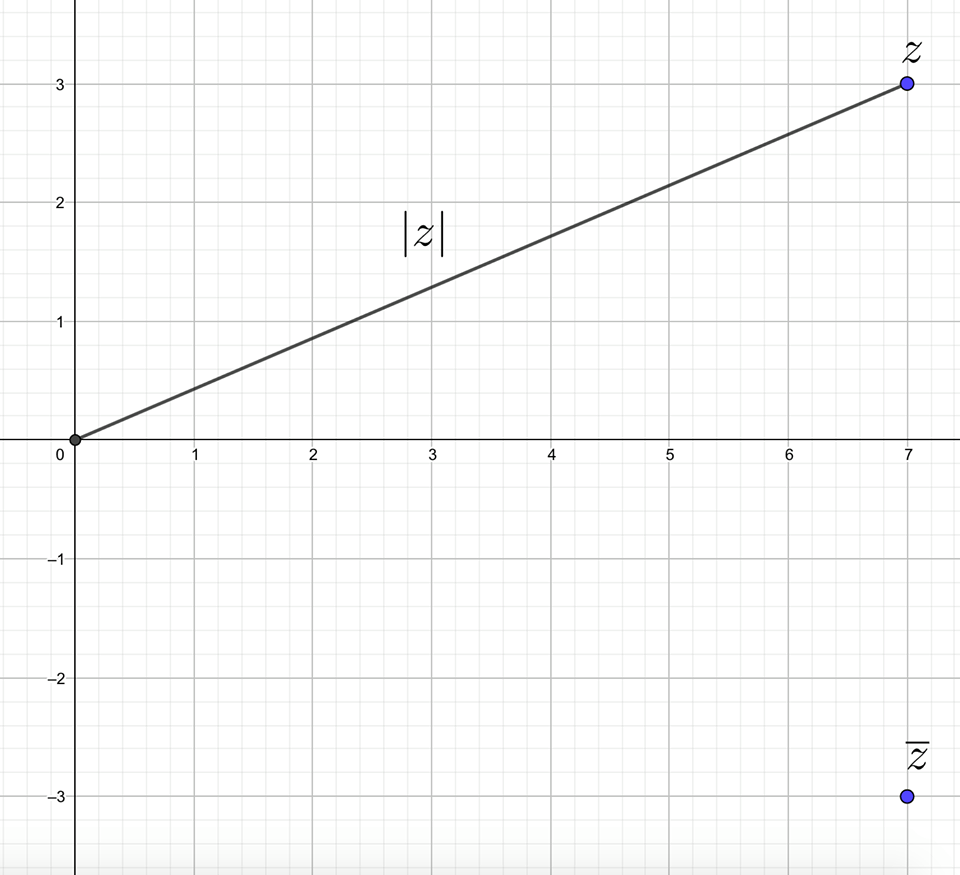
\includegraphics[scale=0.2]{fig/img/complex_plan}
\caption{The complex plane with the number $z=7+3i$, its conjugate $\bar{z}=7-3i$, and $|z|$}
\end{figure}

%RETTET HERTIL

\section{Adding and Subtracting}
When adding complex numbers the imaginary unit $i$, can be treated as a variable like in classic algebra. For instance, if you have something like $(5+2i)+(9+8i)$ then you can add the imaginary parts and the real parts and put it together on the general form; $a+bi$. In this case, we get $14+10i$. This rule can be explained in a general form: 
\begin{align*}
(a + bi) + (c + di) = (a + c) + i(b + d)
\end{align*}
Subtracting is similar because you can only subtract a imaginary part from another imaginary part, and the same goes for the constants. Here is an example:
\begin{align*}
(21 + 3i) - (2 - 2i) = 21 + 3i - 2 + 2i = 19 + 5i
\end{align*}
Similarly this can be put in a general form:
\begin{align*}
(a + bi) - (c + di) = (a - c) + i(b - d)
\end{align*}
From the examples above we can see that subtracting and adding with complex numbers is identical to subtracting and adding other and more familiar variables such as $x$, $y$ etc.

\section{Multiplying}
When multiplying complex numbers, the fact that $i^2 =-1$ must be taken into account. However the multiplication of complex numbers can still be generalized. 
\begin{definition}{Multiplying complex numbers}{def:MCN}
The product of two complex numbers $z_1=a+ib$ and $z_2=c+id$ has the general form:
\begin{align*}
(a+ib)(c+id)&=a(c+di)+ib(c+di)
\\
&=ac+adi+bci+bdi^2
\\
&=(ac-bd)+i(ad+bc)
\end{align*}
\end{definition}
\begin{example}{Multiplying complex numbers}{}
Given two complex numbers $z_1=3+5i$ and $z_2=4-3i$ the product can found using \Cref{def:MCN}
\begin{align*}
(3+5i)(4-3i) = (3\cdot4-5\cdot(-3))+i(3\cdot(-3)+5\cdot4)=27+11i
\end{align*}
\end{example}


\section{Dividing}
When dividing with a complex number the aim is to get some values we can put on the general form $a + bi$. 
\begin{definition}{Dividing complex numbers}{def:DCM}
Division of two complex numbers where $z_1=a+ib$ and $z_2=c+id$ has the general form
\begin{align*}
\frac{a + bi}{c + di} 										
&= \frac{(a+bi)(c-di)}{(c+di)(c-di)} 						\\[1em]
&= \frac{a(c-di)+bi(c-di)}{a^2+b^2} 							\\[1em]
&= \frac{ac-adi+bci-bdi^2}{a^2+b^2}							\\[1em]
&= \frac{(ac+bd)+i(bc-ad)}{a^2+b^2}							\\[1em]
&= \frac{ac+bd}{a^2+b^2}+i \frac{bc-ad}{a^2+b^2}				
\end{align*}
\end{definition}
\begin{example}{Dividing complex numbers}{}
Given two complex numbers $z_1=18+10i$ and $z_2=3+2i$ can be found using \Cref{def:DCM}:
\begin{align*}
\frac{18 + 10i}{3 + 2i} &= \dfrac{18\cdot3+10\cdot2}{18^2+10^2}+i\dfrac{10\cdot3-18\cdot2}{18^2+10^2}
\\
&=\dfrac{37}{9}-\dfrac{1}{3}i
\end{align*}
\end{example}
From the example $\frac{37}{9} - \frac{1}{3}i$ is now on the form $a+ib$ with a and b being fractions. In the example the denominator is being conjugated and as a result of that the imaginary part of the denominator $ib$ disappears and is only left in the numerator. 
\section{Complex Numbers in Polar form}
A complex number $z=a+ib$ in polar form is written on the form $(r,\theta)$, where $r$ is the distance from origin to the point $z$. $\theta$ is the angle from the real axis, when measured counter-clockwise. The angle of a complex number is denoted as $\arg(z)=\theta$.
of this is shown in the figure \ref{fig:complex_plane_polar} below.
\begin{figure}[H] 
\centering
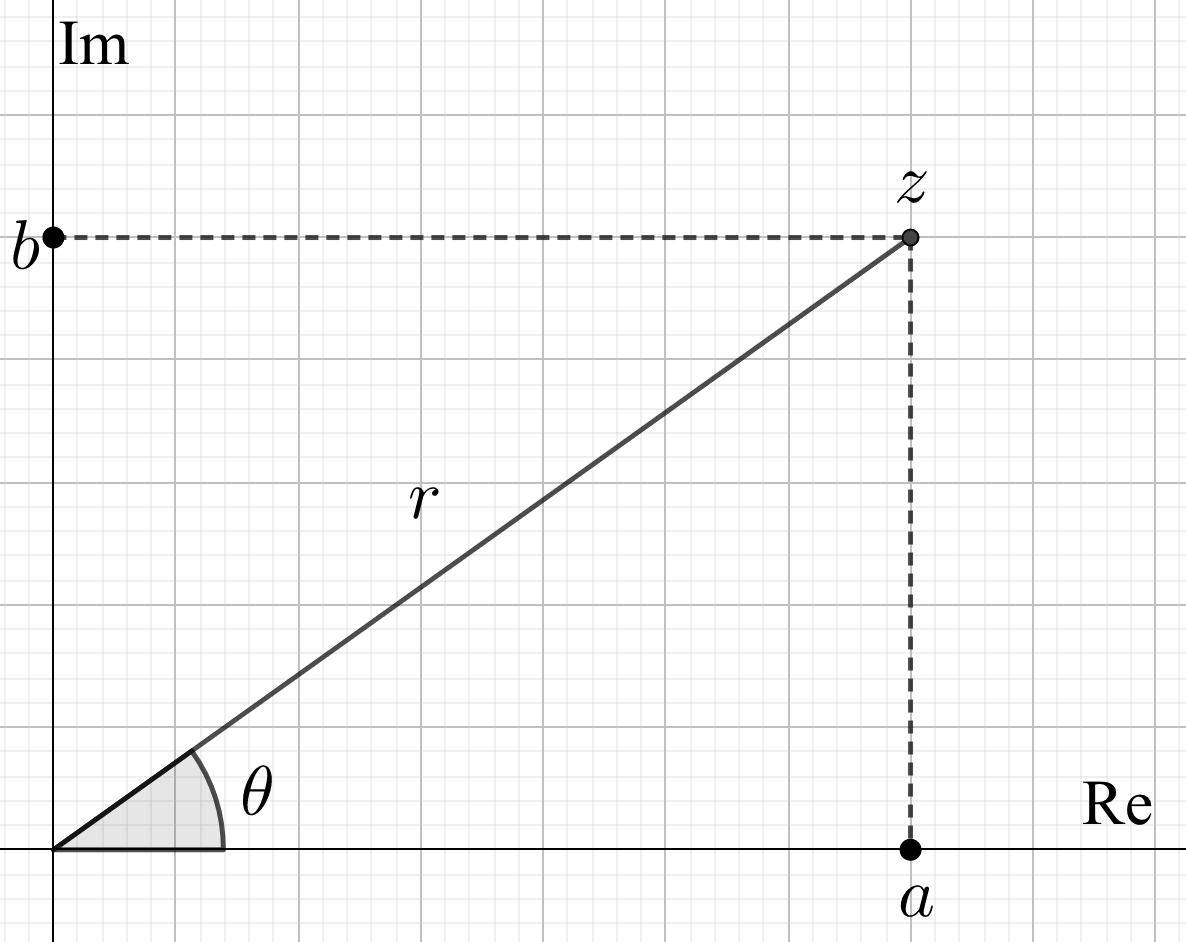
\includegraphics[scale=0.15]{fig/img/complex_plan_polar}
\caption{The complex plane with $z=a+ib$ plotted in terms of polar coordinates and Cartesian coordinates}
\label{fig:complex_plane_polar}
\end{figure}
\noindent
It can be derived from \ref{fig:complex_plane_polar} that the coordinates of $z=a+ib$ can be expressed as follows:
\begin{align}
\text{Re}\{z\}=r\cos(\theta)
\\
\text{Im}\{z\}=r\sin(\theta)
\end{align}
\\
\begin{definition}{Complex number in polar form}{}
A complex number $z=a+ib$ can be written in polar form as follows:
\begin{align}
z&=r\cos(\theta)+ir\sin(\theta)
\\
&=r\left(\cos(\theta)+i\sin(\theta)\right).
\end{align}
Where $r=\mid z \mid$ and $\theta=\tan^{-1}\left(\dfrac{b}{a} \right)$
\end{definition}
\begin{theorem}{Multiplication in polar form}{complex:multi}
Given two complex numbers $z_1$ and $z_2$ where.
\begin{align*}
z_1=r_1(\cos(\theta_1)+i\sin(\theta_1)) 
\\
z_2=r_2(\cos(\theta_2)+i\sin(\theta_2))
\end{align*}
The multiplication of these are given by
\begin{align*}
z_1 z_2=r_1r_2\left( \cos(\theta_1+\theta_2)+ i \sin(\theta_1+\theta_2)\right)
\end{align*}
From this the following relations can be concluded:
\begin{align}
\arg(z_1z_2)&=\arg(z_1)+\arg(z_2)
\\
|z_1z_2|&=|z_1||z_2|
\end{align}
\end{theorem}
\begin{prof}{Multiplication in polar form}{}
\begin{align}
z_1 z_2&=r_1( \cos(\theta_1)+ i \sin(\theta_1))r_2( \cos(\theta_2)+ i \sin(\theta_2)) \nonumber
\\
\label{polar_multiplication}
z_1z_2&=r_1r_2\left( (\cos(\theta_1)\cos(\theta_2)-\sin(\theta_1) \sin(\theta_2))+i(\cos(\theta_1)\sin(\theta_2)+\sin(\theta_1)\cos(\theta_2)\right)
\end{align}
From trigonometry, sine of a sum and cosine of a sum can be expressed as:
\\
\begin{align} \label{sum_cos_sin}
\sin(\theta_1+\theta_2)=\cos(\theta_1)\sin(\theta_2)+\sin(\theta_1)\cos(\theta_2)
\end{align}
\begin{align*}
\cos(\theta_1+\theta_2)=\cos(\theta_1)\cos(\theta_2)-\sin(\theta_1)\sin(\theta_1)
\end{align*}
\\
These definitions are inserted in \eqref{polar_multiplication}.
\\
\begin{align*}
z_1 z_2=r_1r_2\left( \cos(\theta_1+\theta_2)+ i \sin(\theta_1+\theta_2)\right)
\end{align*}
\end{prof}
\begin{theorem}{Division in polar form}{}
Given two complex numbers
\begin{align*}
z_1=r_1(\cos(\theta_1)+i\sin(\theta_1)) 
\\
z_2=r_2(\cos(\theta_2)+i\sin(\theta_2))
\end{align*}
The division of these are given by:
\begin{align*}
\dfrac{z_1}{z_2}=\dfrac{r_1}{r_2}\Big( \cos(\theta_1-\theta_2)+ i \sin(\theta_1-\theta_2)\Big)
\end{align*}
From this the following relations can be concluded:
\begin{align}
\arg\Big(\dfrac{z_1}{z_2}\Big)&=\arg(z_1)-\arg(z_2)
\\
\Big|\dfrac{z_1}{z_2}\Big|&=\dfrac{|z_1|}{|z_2|} \label{eq:mod_div}
\end{align}
\end{theorem}
\begin{prof}{}{}
\begin{align}
\dfrac{z_1}{z_2}&=\dfrac{r_1\bigg(\cos(\theta_1)+i\sin(\theta_1)\bigg)}{r_2\bigg(\cos(\theta_2)+i\sin(\theta_2)\bigg)}
\end{align}
Multiply both sides by $r_2\bigg(\cos(\theta_2)-i\sin(\theta_2)\bigg)$
\begin{align}
\dfrac{z_1}{z_2}&=\dfrac{r_1\bigg(\cos(\theta_1)+i\sin(\theta_1)\bigg)r_2\bigg(\cos(\theta_2)-i\sin(\theta_2)\bigg)}{r_2\bigg(\cos(\theta_2)+i\sin(\theta_2)\bigg)r_2\bigg(\cos(\theta_2)-i\sin(\theta_2)\bigg)}
\end{align}
From \Cref{complex:multi} this can we rewritten as:
\begin{align}
\dfrac{z_1}{z_2}&=\dfrac{r_1r_2\bigg(\cos(\theta_1-\theta_2)+i\sin(\theta_1-\theta_2)\bigg)}{{r_2}^2\bigg(\cos(\theta_2-\theta_2)+i\sin(\theta_2-\theta_2)\bigg)}
\\
&=\dfrac{r_1}{r_2}\Big( \cos(\theta_1-\theta_2)+ i \sin(\theta_1-\theta_2)\Big)
\end{align}
\end{prof}
\section{The Complex Exponential Equation}
The concept of the complex exponential function is useful in circuit analysis. However it must be defined, as it is not entirely obvious what $e$ raised to a complex number means.
\\
\\
For the complex exponential function to be useful for this context, it needs to fulfill two conditions:
\begin{itemize}
	\item $e^{z_1}e^{z_2} = e^{z_1 + z_2}$
	\item $\dfrac{d}{dt}e^{zt} = ze^{zt}$
\end{itemize}
The complex exponential function can be defined as follows, and it can be show that this definition, will satisfy the given conditions.

\begin{definition}{The complex exponential equation}{}
Any complex number can be expressed in the form:
\begin{align*}
	z \cdot t = (a + ib)t,
\end{align*}
where $a,~b,~and~t$ are real numbers, and $i$ is the imaginary unit.
\\
\\
The complex exponential function is then defined as:
\begin{align*}
	f(t)=e^{zt}=e^{at}e^{ibt}=e^{at}\left(\cos(bt)+i\sin(bt)\right)
\end{align*}
\end{definition}
\noindent
Given this definition of the complex exponential function, it can then be shown that the conditions set earlier will hold.
\begin{theorem}{Multiplication of complex numbers in exponential form}{}
Given two complex numbers in exponential form $e^{z_1}$ and $e^{z_2}$ where:
\begin{align*}
z_1=a_1+ib_1
\\
z_1=a_2+ib_2
\end{align*}
The product of the two complex numbers is given by:
\begin{align*}
e^{z_1}e^{z_2}=e^{z_1+z_2}
\end{align*}
\end{theorem}
\begin{prof}{}{}
From definition 5.4 %skal ændres%
the product can be written as.
\begin{align*}
e^{z_1}e^{z_2}&=e^{a_1}(\cos(b_1)+i\sin(b_1))e^{a_2}(\cos(b_2)+i\sin(b_2))
\\
&=e^{a_1}e^{a_2}\left( (\cos(b_1)\cos(b_2)-\sin(b_1) \sin(b_2))+i(\cos(b_1)\sin(b_2)+\sin(b_1)\cos(b_2)\right)
\end{align*}
From \eqref{sum_cos_sin} this can be rewritten as:
\begin{align*}
&=e^{a_1}e^{a_2}(\cos(b_1+b_2)+i(\sin(b_1+b_2))
\end{align*}
Since both $e^{a_1}$ and $e^{a_2}$ are real numbers, their exponents can be added.
\begin{align*}
&=e^{a_1+a_2}(\cos(b_1+b_2)+i(\sin(b_1+b_2))
\end{align*}
From definition 5.4 %skal ændres
this can rewritten as:
\begin{align*}
&=e^{a_1+a_2}e^{i(b_1+b_2)}
\\
&=e^{a_1+ib_1}e^{a_2+ib_2}
\\
&=e^{z_1+z_2}
\end{align*} 
\end{prof}
\begin{theorem}{Differentiating a complex exponential function}{}
Given the complex function:
\begin{align*}
f(t)=e^{zt}=e^{at}(\cos(bt)+i\sin(bt))
\end{align*}
Where $z=a+ib$. The differentiation of this function is given by:
\begin{align*}
\dfrac{d}{dt}e^{zt}=ze^{zt}
\end{align*}
\end{theorem}
\begin{prof}{}{proof:complex:diff:exp}
To show that the function $f(t)=e^{z t}$ is differentiable, where $z=a+ ib$:
\begin{align*}
	f(t) = e^{zt}= e^{(a+ib)t}= e^{at}  e^{ib t}.
\end{align*}
The imaginary part of the complex number $e^{ib\cdot t}$ can be rewritten using \cref{eulers_form}:
\begin{align*}
	f(t) =& e^{at}\big(\cos(bt)+i \cdot \sin(bt)\big), \\
		 =& e^{at}\cos(bt) + e^{at} i \cdot \sin(bt).
\end{align*}
The rewritten function can be differentiated using the chain rule:
\begin{align}
	\dfrac{d}{dt}f(t) =& ae^{at}\cos(bt) -ib \cdot \sin(bt)e^{at} + ia \cdot e^{at}\sin(bt) + ib \cdot e^{at}\cos(bt), \nonumber \\
	=& e^{at} \bigg( a\big(\cos(bt) + i \cdot \sin(bt)\big) + b\big(i \cdot \cos(bt) - \sin(bt)\big) \bigg), \nonumber \\
	=& e^{at}\bigg(a \cdot e^{ib \cdot t}+b\big(i \cdot \cos(bt) - \sin(bt)\big)\bigg), \nonumber \\
	=& a e^{t(a+ib)} + b e^{at}\big(i \cdot \cos(bt) - \sin(bt)\big). \label{proof:chain}
\end{align}
Since $i^2 = -1$, \eqref{proof:chain} can be rewritten. Furthermore, $a+ib$ is replaced with $z$:
\begin{align*}
	\dfrac{d}{dt}f(t) =& a e^{zt} + b e^{at}\big(i \cdot \cos(bt) + i^2 \cdot \sin(bt)\big).
\end{align*}
$i$ is now moved outside the parentheses, and \cref{eulers_form} is used to reduce the equation:
\begin{align*}
	\dfrac{d}{dt}f(t) =&  a e^{zt} + ib e^{at}\big(\cos(bt) + i \cdot \sin(bt)\big), \\
	=&  a e^{zt} + ib e^{at}e^{ib \cdot t}. \\
\end{align*}
Now $a+ib$ is replaced with $z$, and $e^{zt}$ can be placed outside of the parentheses:
\begin{align*}
	\dfrac{d}{dt}f(t) =&  a e^{zt} + ib e^{t(a+ib)}, \\
	=&  e^{zt}(a+ib).
\end{align*}
$a+ib$ is again replaced with $z$, and \cref{theorem:complex:exp} is proved.
\end{prof}

\noindent
It is then shown that the given definition for the complex exponential function, the conditions we set will hold.